\section{Comm. Basics}
\redtext{ISO OSI:}
Open Systems Interconnection model, 
Basis for standards development on SY interconnection,
Reference model.
\textbar
\redtext{Layers:}
\bluetext{
Application(Peer protocol: HTTP, DNS, FTP);
Presentation;
Session;
Transport: TCP/UDP;
Network: IP;
Data link;
Physical}
\\ 
\redtext{IPv4 v6(no checksum):}
Relays datagrams accross networks,
Routing enables internetworking,
Deliver packet from source to host address,
Foundation for TCP/UDP
\\
\redtext{IP routing:}routing protocol,
\bluetext{BGP} used in internet:
Border Gateway Protocol,
Routing between AS (Autonomous systems, provider or bigger organization),
Exchanges routing and reachability information between AS.
\\
\redtext{TCP:} for \bluetext{HTTP, RPC},
Slower than UDP, but with reliability using ACK,
Connection oriented protocol, session is initiated,
Provides ordering, sequencing,
Flow control, sender can't overflow receiver(same speed sending, receiving),
PortNum in TCP protocol(not in IP protocol)
\\
\redtext{UDP:} for \bluetext{DNS, Video, Voice},
Faster than TCP,
Connectionless(no session);
Best-effort;
Packet independent; 
No guaranteed delivery;
No ordering guarantees;
P2P and P2-multipoint.
\\
\redtext{Ports:}
a 16 bit number to local host to identify the connection, 
to differentiate APPs, if packet arrive;
Separate for \bluetext{UDP and TCP};
$0-1023$ reserved to root,
$1024 - 65535$  available to regular user;
http 80/tcp, ftp 21/tcp, ssh 22/tcp, telnet 23/tcp, finger 79/tcp, snmp 161/udp
\\
\redtext{APP Layer protocol:}
Set of rules specifying data transfer
between computing end-points
(Connection establishment \& tear-down
Data representation,
Comm);
\bluetext{DHCP} (Dynamic Host Configuration Protocol),
\bluetext{HTTP} (Hypertext Transfer Protocol),
\bluetext{FTP} (File Transfer Protocol),
\bluetext{Telnet} (Telnet Remote Protocol),
\bluetext{SSH} (Secure Shell Remote Protocol),
\bluetext{SIP} (Session Initiation Protocol),
\bluetext{POP3} (Post Office Protocol 3),
\bluetext{SMTP} (Simple Mail Transfer Protocol),
\bluetext{IMAP} (Internet Message Access Protocol),
\textbar \textbar
browser retreives web page(HTTP 1.1 over TCP, HTTP, FTP, SMTP)
\\
\redtext{HTTP/1.0 C S:}
\bluetext{Request}: GET <path>/index.html HTTP/1.0
\bluetext{Response}: HTTP/1.0 200 OK
\bluetext{ErrorResponse}: HTTP/1.0 404 Not Found 
\textbar \textbar
\redtext{HTTP/1.1:}
HyperText Transfer Protocol,
Request/Response protocol for C S comm. on top of TCP
(Browser,
RESTFUL API‘s,
SOAP over HTTP,
NoSQL databases)
\bluetext{Methods:}
\bluetext{GET:}cacheable get info by Request-URI
\bluetext{HEAD:} like GET but MUST NOT return a message-body
\bluetext{POST:} post a form (bulletin board), uploading data,
can be a data-accepting process
Responses not cacheable(200 (OK), 204(No Content), 201
(Created), 303 (See Other)) 
\bluetext{PUT:} Enclosed entity to be stored under Request-URI
Responses not cacheable
\bluetext{DELETE:} Delete the resource by Request-URI
Response: 200 (OK), 202 (Accepted), 204 (No Content)
\bluetext{TRACE:} for diagnostics
\bluetext{CONNECT:} to initialize secure connection, HTTPS on port 443,
Proxy is asked to forward the TCP connection
\textbar
\redtext{HTTP/1.1 proxy:}C \bluetext{GET req.} $\rightarrow$ Proxy, but not in cache. 
Proxy \bluetext{GET req.} $\rightarrow$ Origin, Origin $\rightarrow$ Proxy response.
C \bluetext{GET req.} $\rightarrow$ Proxy, Proxy $\rightarrow$ C cached resp.
\textbar
\redtext{HTTP/2.0:}
Better utilization network capacity,
Headers compressed,
On a single connection req and resp interleaved,
Prioritization of requests
% FIXME: can be removed
\textbar \textbar \textbar
GET/HTTP/1.1
Host:www.tum.de
Connection:keep-alive
Accept: text/html,application/xhtml+xml,application/xml;q=0.9, image/webp, */*;q=0.8
User-Agent: Mozilla/5.0 (X11; Linux x86\_64) AppleWebKit/537.36 (KHTML, like Gecko) Chrome/37.0.2062.120 Safari/537.36
Accept-Encoding: gzip,deflate,sdch
\textbar \textbar \textbar
HTTP/1.1 200 OK
Date: Wed, 08 Oct 2014 15:25:53 GMT
Server: Apache
X-Powered-By: PHP/5.5.17
Content-Encoding: gzip
%
%
%
\\
\mysubsection{Socket}
\\
Move data/Msg/(invoke operation/service and return result/failure) 
from APP I on Host A to APP K on Host B.
\redtext{Client}:Issues req to S(send \& receive).
\redtext{Server}:Starts up and listens for connections, req.s, and sends/receives.
\redtext{C S eg.}: \bluetext{P2P} telnet/telnetd, ftp/ftpd (sftp/sftpd), Firefox/Apache.
\\
\rtext{Socket}: using network API, network programming abstraction for comm. among processes (APPs) based on (Unix) file
descriptors.
\bluetext{File/Socket descriptor}:int for open file managed by the OS, 
In \orangetext{Unix any I/O} by reading/writing from/to file descriptors.
\textbar
\redtext{Socket types}: 
\bluetext{Stream socket:}telent, HTTP, browser, java.net.ServerSocket, TCP based(Ordering guaranteed, Error-free); 
\bluetext{Datagram socket:}java.net.DatagramSocket, UDP based; 
\bluetext{IPv4\&IPv6}
\\
\redtext{2 end-points determine a connection}: IP address (host address)$+$Port number
\\
\rtext{SetUp,UseSockets}
\orangetext{S Create:}
\lstinline{final ServerSocket ss=new;/*localhost only*/ss.bind(new InetSocketAddress("0.0.0.0", port));while(true){Socket c=ss.accept();/*Block till C*/}
\orangetext{C connect S:}
\lstinline{Socket s = new;s.connect(new InetSocketAddress("127.0.0.1", port));PrintWriter output=new(s.getOutputStream());BufferedReader input=new(new InputStreamReader(s.getInputStream()));output.write(req + "\r\n");/*to S*/output.flush();}
\orangetext{S handle req.:}
\lstinline{/*in while true*/BufferedReader in=new(new InputStreamReader(clientSocket.getInputStream(),Constants.TELNET_ENCODING));PrintWriter out=new(new OutputStreamWriter(clientSocket.getOutputStream(),Constants.TELNET_ENCODING));String firstLine;while((firstLine=in.readLine())!=null)/*req from C*/String res=kv.process(firstLine);out.write(res);/*to C*/out.flush();}
\orangetext{C read resp.:}
\lstinline{/*after C connect S*/String response=input.readline();s.close();}
\orangetext{S shutdown:}
\lstinline{ss.close();}
\adjincludegraphics[width=1\linewidth, trim={0 0 0 {.12\height}},clip]{chap1_1.png}
\redtext{\hlgray{Finite state machines FSM}} \hlgray{describing} 
\redtext{\hlgray{a comm. session C S}}.
\hlgray{C\&S keep comm. session open and exchange Msg until one of them closed.}
\orangetext{\hlgray{accept:}} \hlgray{a} \lstinline{while loop}:
\orangetext{\hlgray{create a new socket (and th.) for commu. with C}}
% \\
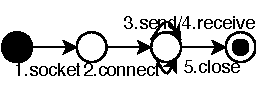
\includegraphics[width=.49\linewidth]{client_FSM.pdf}
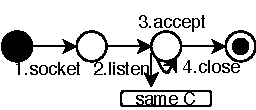
\includegraphics[width=.49\linewidth]{server_FSM.pdf}
\rtext{K V Server:} C get, set Table in S: 
\bluetext{PUT tablename key value\textbackslash r\textbackslash n}, 
\bluetext{GET tablename key}
\textbar
\redtext{C:}
\orangetext{C.java:}
\lstinline{KVTable<AssessmentInformation> kvc=new;kvc.put("middleware" new AssessmentInformation(1.3);}
\orangetext{KVTable.java in put():}
\lstinline{String jsonStr=gs.toJson(value);String enc_value=encodeBase64(jsonStr);this.activeConnection.write("PUT "+this.table+" "+key+" "+enc_value+"\r\n");}
\orangetext{ActiveConnection.java in write():}
\lstinline{PrintWriter output...;output.write(..);output.flush();}
\redtext{S:}
\orangetext{ConnectionHandleThread.java}
\lstinline{BufferedReader in=new(new ISReader(clientSocket.getIS(),...));String line=in.readLine();}
\orangetext{KVStore.java}
\lstinline{StringTokenizer st=new(firstLine," \r\n");String command=st.nextToken();if(command=="GET")/*GET PUT else*/}
\orangetext{ConnectionHandleThread.java}
\lstinline{PrintWriter out = new PrintWriter(new OutputStreamWriter(clientSocket.getOutputStream(),...));out.write(res);/*to C*/out.flush();}
\\
\rtext{\hlgray{Sequence Dia multi th:}}
\btext{\hlgray{n times C and Th.}}
\textbar
\bluetext{\hlgray{Ci to S:}} \hlgray{connect}, 
\bluetext{\hlgray{S to Th.i}}, 
\bluetext{\hlgray{Ci to S to Th.i:}} \hlgray{getTime()},
\bluetext{\hlgray{Th.i to S to C:}} \hlgray{20:00}
\\
\rtext{\hlgray{S Create:}} 
\hlgray{same as single th. above}
\orangetext{\hlgray{S Create}}
\bluetext{\hlgray{instead of block IO in while:}}
\lstinline{public void provideService(){int port=8883;ServerSocket s=new();s.listen(port);while(true){Socket c=s.accept();HandleRequest hr=new(client);hr.start();}  
\\
\rtext{\hlgray{HandleRequest as Th.:}}
\lstinline{class HandleRequest extends Thread{private Socket c;HandleRequest(Socket c){c=c;/*]*/run(){String msg=c.receive()if(msg=="getTime"){String res=getTime();c.send(res);c.close();}
\\
\rtext{\hlgray{C:}}
\lstinline{class Client{public void sendMessage(){String ip="112.32.86.113";int port=8883;String msg="getTime";Socket c=new();c.connect(ip,port);c.send(msg);String res=c.receive();c.close();print res;}
\mysubsection{NIO(NonblockingSockets),multi.threaded}
\\
\redtext{Synchronous}: 
Single th. read data from C(stream) and blocked until done
\rtext{Asynchronous}: 
th. $\rightarrow$ \bluetext{Channel}: 
read data into \bluetext{Buffer}; 
\bluetext{Channel} $\rightarrow$ \bluetext{Buffer}: 
fill data into \bluetext{Buffer}; 
Th. $\rightarrow$ \bluetext{Buffer}: 
check data in \bluetext{Buffer} (main th. not blocked)
\\
\rtext{\hlgray{Syn. vs. Asyn.}}: 
\bluetext{Syn}: Th. acts and waits until \orangetext{Syn. I/O} done; 
\orangetext{}text{Limited scalability}, a th. per I/O connection
(Overhead:\orangetext{context switching} $\rightarrow$ time between diff. tasks)
\bluetext{Asyn}: Pass req. to OS-kernel and do other tasks 
$\rightarrow$\orangetext{worker th.}\lstinline{while(true)} 
\rtext{++:}
\orangetext{\hlgray{only Compute, never Blocked, no Context Swtich, Asyn. I/O}}
\hlgray{
Scalability, 
Consumers not block S long time,
One th. handle multi. sockets
}
\rtext{--:}
\hlgray{
Complex handling code,
Requires different kind of architecture(Eventloops)
}
\\
\rtext{Java NIO Channels}: 
All \orangetext{I/O operations} done with \bluetext{channels(File, TCP, UDP)};
Multi types of \bluetext{channels}
(FileChannel(File on disk), 
DatagramChannel (UDP), 
SocketChannel (TCP, support concurrent read/write), 
ServerSocketChannel (TCP));
Responsibility(\orangetext{Read, write buffer})
\\
\rtext{\hlgray{Sequence Dia single th:}}
\btext{\hlgray{n times C}}
\textbar
\bluetext{\hlgray{Ci to S:}} \hlgray{connect}, 
\bluetext{\hlgray{Ci to S:}} \hlgray{getTime()},
\hlgray{all C sent, S start with Zeitraum to process n req.}
\bluetext{\hlgray{Th.i to S to C:}} \hlgray{20:00 resp. same order as sent req.}
\\
\orangetext{\hlgray{handleRequest():}}
\lstinline{public byte[] handleRequest(byte[] input){return Bytes.toBytes(System.nanoTime());}
\redtext{\hlgray{Selector:}} 
\hlgray{select multi asyn. Channels to match a EventLoop}
\orangetext{\hlgray{Setup channel:}}
\lstinline{Hashmap<SocketChannel,byte[]>pendingData;ServerSocketChannel ssc=new();ssc.connect("127.0.0.1",8883);Selector selector=new();ssc.register(selector,SelectionKey.ACCEPT);}
\rtext{!OR!}
\lstinline{ServerSocketChannel ssC=SSC.open();ssC.configureBlocking(false);InetSocketAddress isa=new ISA(InetAddress.getByName("localhost"),5559);ssC.socket().bind(isa);}
\orangetext{\hlgray{Eventloop:}}
\lstinline{public void start() throws IOException{while(true) try{selector.select();/*get List*/Iterator selectedKeys=selector.selectedKeys().iterator();while(selectedKeys.hasNext()){SelectionKey key=(SelectionKey)selectedKeys.next(); selectedKeys.remove();if(key.isAcceptable()){ServerSocketChannel channel=(SSC)key.channel();SocketChannel sC=channel.accept();sC.configureBlocking(false);sC.register(this.selector,SelectionKey.READ);/*wake up when sth to read*/else if(key.isReadable()){SocketChannel channel=(SC)key.channel();byte[] res=handleRequest(channel.read());pendingData.add(channel,res);key.interesOps(SelectionKey.WRITE);else if(key.isWritable()){SocketChannel channel=(SC)key.channel();data=pendingData.get(channel); if(data==(byte[])"getTime"){channel.write((byte[])getTime());key.interestOps(SelectionKey.READ); catch (e){e.printStackTrace();}
% \orangetext{Register selector:}
% \lstinline{Selector s = SelectorProvider.provider().openSelector(); serverChannel.register(s, SelectionKey.OP_ACCEPT); private void accept(SelectionKey key) throws IOException {ServerSocketChannel sSC = (SSC) key.channel(); SocketChannel sC = sSC.accept(); sC.configureBlocking(false); sC.register(this.s, SelectionKey.OP_READ);/*wake up when sth to read*/}
\orangetext{Read:}
\lstinline{private void read(SelectionKey key) throws IOException{SocketChannel sC=(SC)key.channel();this.readBuffer.clear();int numRead=sC.read(this.readBuffer);/*in Buffer*/if(numRead==-1){key.channel().close();key.cancel();return;/*]*/byte[] dataCopy=new byte[numRead];arraycopy(this.readBuffer.array(),0,dataCopy,0,numRead);handleRequest(sC,dataCopy);}
\orangetext{Write:}
\lstinline{private void write(SelectionKey key) throws IOException{SocketChannel sC=(SC)key.channel();List queue=(List)this.pendingData.get(sC);while(!queue.isEmpty()){ByteBuffer buf=(ByteBuffer) queue.get(0);socketChannel.write(buf);if(buf.remaining()>0){break;/*]*/queue.remove(0);/*]*/if(queue.isEmpty()){key.interestOps(SelectionKey.OP\_READ);/*]*/}
\\
\redtext{\hlgray{Protocol Design:}}
\hlgray{complex number as string: c=(a,b,n)}, 
$n \in {s,p}$,
$op \in \{add, sub, mul, div, poloar\}$,
\orangetext{\hlgray{C to S req.:}}\hlgray{m<c1;c2;op>, 
<(1.0,1.0,s);(2.0,4.0,s);add>
Status:} $st\in\{OK,msgIncomplete.msgFormatError,serverError\}$,
\orangetext{\hlgray{S to C resp.:}}
\hlgray{m2<Cr; st>, 
<(3.0,5.0,s); ok>}
\textbar
\redtext{\hlgray{Sequence Dia.:}}
\hlgray{C2S: m1<(a1,b1);(a2,b2);".add">} 
\redtext{+}
\hlgray{S2C:m2<(a1+a2,b1+b2);".ok">;
C2S: m1<(a1,b1);(a}
\redtext{+}
\hlgray{m2<(0.0,0.0);"msgIncomplete">}
\orangetext{\hlgray{execution error, processing correct}}